% Auto-generated by gen_overview.py (v2) -- EGDR overview (one column).
% Needs: \usepackage{tikz}\usetikzlibrary{shadows,positioning,calc,arrows.meta}; amssymb (loaded by wacv.sty)
\definecolor{ovRisk}{RGB}{86,128,186}\definecolor{ovEnt}{RGB}{150,84,160}\definecolor{ovInj}{RGB}{230,126,34}
\definecolor{ovGrayFill}{RGB}{243,244,247}\definecolor{ovGrayLine}{RGB}{190,197,210}\definecolor{ovPrompt}{RGB}{214,214,214}
\definecolor{ovGreenFill}{RGB}{237,247,237}\definecolor{ovGreenLine}{RGB}{150,200,150}
\definecolor{ovBoxLine}{RGB}{160,166,180}\definecolor{ovHal}{RGB}{204,0,0}\definecolor{ovHalBg}{RGB}{255,175,175}
\definecolor{ovGnd}{RGB}{20,110,40}\definecolor{ovGndBg}{RGB}{190,235,190}
\providecommand{\ovhal}[1]{{\setlength{\fboxsep}{0.3pt}\colorbox{ovHalBg}{\textcolor{ovHal}{\textbf{#1}}}}}
\providecommand{\ovgnd}[1]{{\setlength{\fboxsep}{0.3pt}\colorbox{ovGndBg}{\textcolor{ovGnd}{\textbf{#1}}}}}
\begin{tikzpicture}[x=1cm,y=1cm,font=\sffamily\fontsize{5.6}{6.7}\selectfont,panel/.style={rounded corners=4pt, line width=0.5pt, drop shadow={opacity=0.15, shadow xshift=0.5pt, shadow yshift=-0.7pt}},blk/.style={rounded corners=2pt, draw=ovBoxLine, fill=white, line width=0.45pt, inner sep=1.6pt, align=center},arr/.style={-{Stealth[length=3pt,width=2.6pt]}, line width=0.55pt, color=black!65},ttl/.style={font=\sffamily\bfseries\fontsize{6.3}{7.5}\selectfont, anchor=north west, inner sep=0pt}]
\begin{scope}\clip[rounded corners=3pt] (0,0) rectangle (1.62,-1.409);\node[inner sep=0pt, anchor=north west] at (0,0) {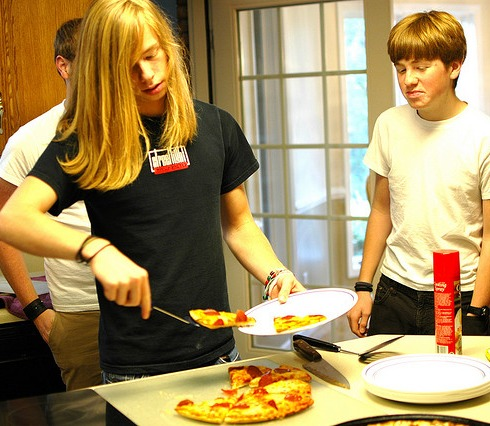
\includegraphics[width=1.62cm]{ov_207108.jpg}};\end{scope}
\draw[rounded corners=3pt, draw=ovBoxLine, line width=0.45pt] (0,0) rectangle (1.62,-1.409);
\node[rounded corners=2pt, fill=ovPrompt, draw=ovPrompt, line width=0.45pt, inner sep=2.4pt, anchor=north west, text width=5.89cm, align=left] (pr) at (2.04,0) {\textbf{Prompt:} Please describe this image in detail.};
\node[blk, anchor=north west, text width=5.89cm, align=center, inner sep=2.4pt] (lv) at (2.04,-0.62) {\textbf{Frozen LVLM} + risk-gated steering at layer $\ell^*$\\[1.6pt]$R_t=-\cos(\mathbf{h}_t,\mathbf{v})>\textbf{gate}\ \Rightarrow\ \mathbf{h}_t\leftarrow\mathbf{h}_t+\alpha\mathbf{v}$\\[1.6pt]{\color{black!70}gate:\ \ (a) constant $\tau$\ \ \textbar\ \ (b) $\tau_{\mathrm{eff}}(t)$}};
\draw[arr] (pr.south) -- (lv.north);
\draw[arr] (1.6700000000000002,-0.824) -- (lv.west |- 0,-0.824);
\draw[panel, fill=ovGrayFill, draw=ovGrayLine] (0,-1.860) rectangle (8.05,-3.880);
\node[ttl] at (0.12,-1.960) {(a) Static gate:\ one constant threshold $\tau$ at every step};
\draw[line width=0.4pt, black!55] (0.46,-3.580) -- (3.605,-3.580);
\fill[ovRisk!60] (0.575,-3.580) rectangle (0.745,-3.105);
\fill[ovRisk!60] (0.880,-3.580) rectangle (1.050,-2.896);
\fill[ovRisk!60] (1.185,-3.580) rectangle (1.355,-3.248);
\fill[ovRisk!60] (1.490,-3.580) rectangle (1.660,-3.058);
\fill[ovRisk!60] (1.795,-3.580) rectangle (1.965,-3.124);
\fill[ovRisk!60] (2.100,-3.580) rectangle (2.270,-2.820);
\fill[ovRisk!60] (2.405,-3.580) rectangle (2.575,-3.181);
\fill[ovRisk!60] (2.710,-3.580) rectangle (2.880,-3.086);
\fill[ovRisk!60] (3.015,-3.580) rectangle (3.185,-3.295);
\fill[ovRisk!60] (3.320,-3.580) rectangle (3.490,-2.953);
\draw[black!60, line width=0.6pt, dash pattern=on 1.6pt off 1.1pt] (0.48000000000000004,-3.010) -- (3.605,-3.010);
\draw[black!45, line width=0.35pt, fill=white] (0.660,-3.020) circle (0.033);
\fill[ovInj] (0.965,-2.811) circle (0.052);
\draw[black!45, line width=0.35pt, fill=white] (1.270,-3.163) circle (0.033);
\draw[black!45, line width=0.35pt, fill=white] (1.575,-2.973) circle (0.033);
\draw[black!45, line width=0.35pt, fill=white] (1.880,-3.039) circle (0.033);
\fill[ovInj] (2.185,-2.735) circle (0.052);
\draw[black!45, line width=0.35pt, fill=white] (2.490,-3.096) circle (0.033);
\draw[black!45, line width=0.35pt, fill=white] (2.795,-3.001) circle (0.033);
\draw[black!45, line width=0.35pt, fill=white] (3.100,-3.210) circle (0.033);
\fill[ovInj] (3.405,-2.868) circle (0.052);
\node[anchor=north west, inner sep=0pt, text=black!60, font=\sffamily\fontsize{4.8}{5.6}\selectfont] at (0.46,-3.630) {$t{=}1$};
\node[anchor=north east, inner sep=0pt, text=black!60, font=\sffamily\fontsize{4.8}{5.6}\selectfont] at (3.605,-3.630) {step $t\rightarrow$};
\node[anchor=east, inner sep=0.5pt, text=ovRisk!80!black, font=\sffamily\fontsize{5}{6}\selectfont] at (0.43000000000000005,-3.152) {$R_t$};
\node[anchor=west, inner sep=0.5pt, text=black!65, font=\sffamily\fontsize{4.8}{5.6}\selectfont] at (3.625,-3.010) {$\tau$};
\node[blk, anchor=north west, text width=3.69cm, align=left, draw=ovGrayLine, fill=white, inner sep=2pt] (b0) at (4.12,-2.200) {\textbf{Static gate:} \ldots\ Several \ovgnd{pizzas} can be seen on the countertops, with some of them being sliced. Kitchen utensils, such as \ovgnd{knives}, \ovhal{forks}, and \ovhal{spoons}, are visible, as well as dining tableware, including \ovhal{forks}, \ovgnd{knives}, and \ovhal{spoons}.\hfill\raisebox{-0.6pt}[0pt][0pt]{\textcolor{ovHal}{\fontsize{8.2}{6.7}\selectfont$\boldsymbol{\times}$}}};
\draw[panel, fill=ovGreenFill, draw=ovGreenLine] (0,-4.080) rectangle (8.05,-7.230);
\node[ttl] at (0.12,-4.180) {(b) EGDR (ours):\ threshold lowered by preceding-step entropy};
\node[blk, draw=ovEnt!70, fill=ovEnt!6, anchor=north west, text width=1.66cm, minimum height=0.60cm, font=\sffamily\fontsize{5.4}{6.4}\selectfont] (c0) at (0.140,-4.480) {logits $\mathbf{q}_{t-1}$\\(already computed)};
\node[blk, draw=ovEnt!70, fill=ovEnt!6, anchor=north west, text width=1.66cm, minimum height=0.60cm, font=\sffamily\fontsize{5.4}{6.4}\selectfont] (c1) at (2.158,-4.480) {entropy $\hat H_{t-1}$\\(Eq.\,4)};
\draw[arr] (c0.east) -- (c1.west);
\node[blk, draw=ovEnt!70, fill=ovEnt!6, anchor=north west, text width=1.66cm, minimum height=0.60cm, font=\sffamily\fontsize{5.4}{6.4}\selectfont] (c2) at (4.175,-4.480) {rescale to band\\$[H_{\mathrm{lo}},H_{\mathrm{hi}}]$:\ $\hat e_t$};
\draw[arr] (c1.east) -- (c2.west);
\node[blk, draw=ovEnt, fill=ovEnt!14, line width=0.6pt, anchor=north west, text width=1.66cm, minimum height=0.60cm, font=\sffamily\fontsize{5.4}{6.4}\selectfont] (c3) at (6.192,-4.480) {$\tau_{\mathrm{eff}}(t)=$\\$\tau-w_\tau\,\hat e_t\,|\tau|$};
\draw[arr] (c2.east) -- (c3.west);
\node[anchor=north east, inner sep=0pt, text=ovEnt!85!black, font=\sffamily\itshape\fontsize{4.9}{5.8}\selectfont] at (7.910000000000001,-5.180) {no extra forward pass, no trained parameter};
\draw[line width=0.4pt, black!55] (0.46,-6.930) -- (3.605,-6.930);
\fill[ovRisk!60] (0.575,-6.930) rectangle (0.745,-6.455);
\fill[ovRisk!60] (0.880,-6.930) rectangle (1.050,-6.246);
\fill[ovRisk!60] (1.185,-6.930) rectangle (1.355,-6.598);
\fill[ovRisk!60] (1.490,-6.930) rectangle (1.660,-6.408);
\fill[ovRisk!60] (1.795,-6.930) rectangle (1.965,-6.474);
\fill[ovRisk!60] (2.100,-6.930) rectangle (2.270,-6.170);
\fill[ovRisk!60] (2.405,-6.930) rectangle (2.575,-6.531);
\fill[ovRisk!60] (2.710,-6.930) rectangle (2.880,-6.436);
\fill[ovRisk!60] (3.015,-6.930) rectangle (3.185,-6.645);
\fill[ovRisk!60] (3.320,-6.930) rectangle (3.490,-6.303);
\draw[black!60, line width=0.6pt, dash pattern=on 1.6pt off 1.1pt] (0.48000000000000004,-6.360) -- (3.605,-6.360);
\draw[ovEnt, line width=0.85pt, line join=round] (0.508,-6.360) -- (0.812,-6.360) -- (0.813,-6.408) -- (1.118,-6.408) -- (1.117,-6.574) -- (1.423,-6.574) -- (1.423,-6.598) -- (1.728,-6.598) -- (1.727,-6.384) -- (2.032,-6.384) -- (2.033,-6.586) -- (2.337,-6.586) -- (2.338,-6.431) -- (2.643,-6.431) -- (2.643,-6.598) -- (2.947,-6.598) -- (2.948,-6.360) -- (3.252,-6.360) -- (3.253,-6.503) -- (3.558,-6.503);
\draw[black!45, line width=0.35pt, fill=white] (0.660,-6.370) circle (0.033);
\fill[ovInj] (0.965,-6.161) circle (0.052);
\draw[black!45, line width=0.35pt, fill=white] (1.270,-6.513) circle (0.033);
\draw[ovInj, line width=0.75pt, fill=white] (1.575,-6.323) circle (0.052);
\draw[black!45, line width=0.35pt, fill=white] (1.880,-6.389) circle (0.033);
\fill[ovInj] (2.185,-6.085) circle (0.052);
\draw[black!45, line width=0.35pt, fill=white] (2.490,-6.446) circle (0.033);
\draw[ovInj, line width=0.75pt, fill=white] (2.795,-6.351) circle (0.052);
\draw[black!45, line width=0.35pt, fill=white] (3.100,-6.560) circle (0.033);
\fill[ovInj] (3.405,-6.218) circle (0.052);
\node[anchor=north west, inner sep=0pt, text=black!60, font=\sffamily\fontsize{4.8}{5.6}\selectfont] at (0.46,-6.980) {$t{=}1$: $\hat e{=}0\Rightarrow\tau_{\mathrm{eff}}{=}\tau$};
\node[anchor=north east, inner sep=0pt, text=black!60, font=\sffamily\fontsize{4.8}{5.6}\selectfont] at (3.605,-6.980) {step $t\rightarrow$};
\node[anchor=east, inner sep=0.5pt, text=ovRisk!80!black, font=\sffamily\fontsize{5}{6}\selectfont] at (0.43000000000000005,-6.503) {$R_t$};
\node[anchor=west, inner sep=0.5pt, text=black!65, font=\sffamily\fontsize{4.8}{5.6}\selectfont] at (3.625,-6.360) {$\tau$};
\node[anchor=west, inner sep=0.5pt, text=ovEnt, font=\sffamily\fontsize{4.8}{5.6}\selectfont] at (3.625,-6.533) {$\tau_{\mathrm{eff}}$};
\fill[ovEnt!70] (0.880,-5.780) rectangle (1.050,-5.720);
\fill[ovEnt!70] (1.185,-5.780) rectangle (1.355,-5.510);
\fill[ovEnt!70] (1.490,-5.780) rectangle (1.660,-5.480);
\fill[ovEnt!70] (1.795,-5.780) rectangle (1.965,-5.750);
\fill[ovEnt!70] (2.100,-5.780) rectangle (2.270,-5.495);
\fill[ovEnt!70] (2.405,-5.780) rectangle (2.575,-5.690);
\fill[ovEnt!70] (2.710,-5.780) rectangle (2.880,-5.480);
\fill[ovEnt!70] (3.320,-5.780) rectangle (3.490,-5.600);
\draw[line width=0.35pt, ovEnt!60] (0.46,-5.780) -- (3.605,-5.780);
\node[anchor=east, inner sep=0.5pt, text=ovEnt!85!black, font=\sffamily\fontsize{5}{6}\selectfont] at (0.43000000000000005,-5.650) {$\hat e_t$};
\node[blk, anchor=north west, text width=3.69cm, align=left, draw=ovGreenLine, fill=white, inner sep=2pt] (b1) at (4.12,-5.400) {\textbf{EGDR:} \ldots\ Several \ovgnd{pizza} slices can be seen on plates, with some of them already being sliced. The room is equipped with a dining \ovgnd{table}, where some of the \ovgnd{teenagers} are standing or seated.\hfill\raisebox{-0.6pt}[0pt][0pt]{\textcolor{ovGnd}{\fontsize{8.2}{6.7}\selectfont$\boldsymbol{\checkmark}$}}};
\begin{scope}[shift={(0.05,-7.430)}]\fill[ovRisk!60] (0,-0.05) rectangle (0.12,0.07);\node[anchor=west, inner sep=0pt, font=\sffamily\fontsize{4.7}{5.6}\selectfont] at (0.18,0.01) {risk $R_t$};\end{scope}
\begin{scope}[shift={(1.00,-7.430)}]\draw[black!60, line width=0.6pt, dash pattern=on 1.6pt off 1.1pt] (0,0.01) -- (0.26,0.01);\node[anchor=west, inner sep=0pt, font=\sffamily\fontsize{4.7}{5.6}\selectfont] at (0.33,0.01) {static $\tau$};\end{scope}
\begin{scope}[shift={(2.18,-7.430)}]\draw[ovEnt, line width=0.85pt] (0,0.01) -- (0.26,0.01);\node[anchor=west, inner sep=0pt, font=\sffamily\fontsize{4.7}{5.6}\selectfont] at (0.33,0.01) {$\tau_{\mathrm{eff}}(t)$};\end{scope}
\begin{scope}[shift={(3.40,-7.430)}]\fill[ovInj] (0.06,0.01) circle (0.052);\node[anchor=west, inner sep=0pt, font=\sffamily\fontsize{4.7}{5.6}\selectfont] at (0.18,0.01) {corrected by both};\end{scope}
\begin{scope}[shift={(5.10,-7.430)}]\draw[ovInj, line width=0.75pt, fill=white] (0.06,0.01) circle (0.052);\node[anchor=west, inner sep=0pt, font=\sffamily\fontsize{4.7}{5.6}\selectfont] at (0.18,0.01) {by EGDR only};\end{scope}
\begin{scope}[shift={(6.60,-7.430)}]\draw[black!45, line width=0.35pt, fill=white] (0.06,0.01) circle (0.033);\node[anchor=west, inner sep=0pt, font=\sffamily\fontsize{4.7}{5.6}\selectfont] at (0.18,0.01) {not corrected};\end{scope}
\end{tikzpicture}
